\documentclass{article}
\usepackage[utf8]{inputenc}
%\usepackage{biblatex}
\usepackage{amssymb}
\usepackage{amsmath}
\usepackage{amsthm}
\usepackage{graphicx}
\usepackage{float}
\usepackage{url}
\usepackage{framed}
\usepackage{booktabs}
\usepackage{enumitem}
\usepackage{extarrows}
\usepackage{subcaption}
\usepackage{epstopdf}
\usepackage{hyperref}
%\usepackage{algorithm}
%\usepackage{algorithmic}
\usepackage[ruled,linesnumbered]{algorithm2e}
\numberwithin{equation}{section}
%\usepackage{BOONDOX-calo}
\title{ Partially coherent ptychography}
%\author{huibinchang }
\date{July 2021}

\begin{document}

\maketitle
\tableofcontents

\section{Models}



\subsection{Coherent model}
\begin{equation}
\label{basic}
f_{j}=\left|\mathcal{F}\left( \mathcal{S}_{j} u  \circ \omega \right)\right|^{2} 
\end{equation}

In a discrete setting, $u \in \mathbb{C}^{n}$ is a 2D image with $\sqrt{n} \times \sqrt{n}$ pixels, $\omega \in \mathbb{C}^{\bar{m}}$ is a localized 2D probe with $\sqrt{\bar{m}} \times \sqrt{\bar{m}}$ pixels.

$f_{j} \in \mathbb{R}_{+}^{\bar{m}}(\forall 0 \leq j \leq N-1)$ is a stack of phaseless measurements. Here $|\cdot|$ represents the element-wise absolute value of a vector, o denotes the elementwise multiplication, and $\mathcal{F}$ denotes the normalized 2 dimensional discrete Fourier transform. Each $\mathcal{S}_{j} \in \mathbb{R}^{\bar{m} \times n}$ is a binary matrix that crops a region $j$ of size $\bar{m}$ from the image $u$.

In practice, as the probe is almost never completely known, one has to solve a blind ptychographic phase retrieval (BP-PR) problem:

 To find $\omega \in \mathbb{C}^{\bar{m}}$ and $u \in \mathbb{C}^{n}$ s.t. $|\mathcal{A}(\omega, u)|=\boldsymbol{a}$,
 
where bilinear operators $\mathcal{A}: \mathbb{C}^{\bar{m}} \times \mathbb{C}^{n} \rightarrow \mathbb{C}^{m}$ and $\mathcal{A}_{j}: \mathbb{C}^{\bar{m}} \times \mathbb{C}^{n} \rightarrow \mathbb{C}^{\bar{m}} \forall 0 \leq j \leq N-1$ are
denoted as follows:

 $\mathcal{A}(\omega, u):=\left(\mathcal{A}_{0}^{T}(\omega, u), \mathcal{A}_{1}^{T}(\omega, u), \ldots, \mathcal{A}_{N-1}^{T}(\omega, u)\right)^{T}$, $\mathcal{A}_{j}(\omega, u):=\mathcal{F}\left(\omega \circ \mathcal{S}_{j} u\right)$
 
and $\boldsymbol{a}:=\left(\boldsymbol{a}_{0}^{T}, \boldsymbol{a}_{1}^{T}, \ldots, \boldsymbol{a}_{N-1}^{T}\right)^{T} \in \mathbb{R}_{+}^{m}$.

\subsection{Specific partially coherent model}
 \label{section:specific models}

\subsubsection{Model1\cite{chang}}
Coherence and vibrations kernels can be combined into one, such that partially coherent ptychography imaging with coherence kernel function $\kappa$ in a continuous setting:
\begin{equation}
f_{p c, j}(q) = \int\left|\mathcal{F}_{x \rightarrow q}\left(\mathcal{S}_{j} u(x) \omega(x-y)\right)\right|^{2} \kappa(y) \mathrm{d} y
\end{equation}

where $f_{p c}$ is the measured partial coherent intensity and $\mathcal{F}_{x \rightarrow q}$ is the normalized Fourier transform. $\kappa$ is a function that spikes at 0 like guassians. Setting $\kappa$ to the Dirac delta function reduces it to the coherent model (\ref{basic}).

The partially coherent intensity in a discrete setting is generated as
\begin{equation}
f_{p c, j}=\sum_{i} \kappa_{i}\left|\mathcal{F}\left( \mathcal{S}_{j} u \circ \left(\mathcal{T}_{i} \omega\right) \right)\right|^{2}
\label{model:target}
\end{equation}


with translation operator $\mathcal{T}_{i}$, discrete Gaussian weights $\left\{\kappa_{i}\right\}$, and periodical boundary condition for the probe.

Generally speaking, solving (\ref{model:target}) is a non-linear
ill-posed problem with an unknown kernel $\kappa$, unknown phobe $\omega$, and unknown target image $u$. 
%\textbf{And it is the main target in this research.}

\subsubsection{Model2\cite{psf}}
Another simpler model mentioned here is:

\begin{equation}
\label{simple}
    f_{p c}=f * \kappa
\end{equation}

where $f_{p c}$ is the measured partial coherent intensity, $f$ is the coherent intensity in (\ref{basic}), $*$ denotes the convolution operator, and $\kappa$ is the unknown kernel function (Fourier transform of the complex coherence function). 



We remark that (\ref{model:target}) is quite different from
 (\ref{simple}) , since (\ref{model:target}) illustrates the effects of blurring of images with respect to the probe, while (\ref{simple}) can be interpreted as blurring or binning multiple pixels at the detector.

\subsection{General partially coherent model}
This part explains the partially coherent model proposed by physicists.\cite{mix}.   It is a blind ptychography model based on quantum state tomography\footnote{\url{https://homepage.univie.ac.at/reinhold.bertlmann/pdfs/T2_Skript_Ch_9corr.pdf}Theorem 9.1. Many symbols in quantum mechanics are included here.}.  Phobe $w$ is assumed to be in a mixed state to represent a partially coherent effect.


\subsubsection{Decompositon model}

 
\begin{equation}
\label{sep} 
\begin{aligned}
&\mbox{Find } u, r \mbox{ othogonal $w_k$   }s.t. \\
&f_{p c, j}=\sum_{k=1}^r \left|\mathcal{F}\left( \mathcal{S}_{j} u \circ \left(\omega_k\right) \right)\right|^{2} (0\leq j \leq N-1)
\end{aligned}
\end{equation}

 


Denote $O_j \in C^{\bar{m} \times \bar{m}}$ as a (diagonal) matrix to represent linear transform to $w$, s.t. $\mathcal{S}_{j} u \circ \omega = O_j w$. Denote $f_q^* \in C^{1 \times \bar{m}}$ as a row vector  constructed from Fourier transform $\mathcal{F}$, to represent projection on frepuency element. Construct measurement matrix $ \mathcal{I}_{j \mathbf{q}} = O_j^*f_qf_q^*O_j$ and density matrix $\rho$, we get another form(actually a natural one in quantum state tomography) of the model:


\begin{equation}
\label{lift}
\begin{aligned}
&\mbox{Find } u,\rho,s.t.\\
&f_{pc,j}(q) = Tr(\mathcal{I}_{j \mathbf{q}} \rho ) (0\leq j \leq N-1)\\
&\rho \mbox{ is positive semi-definite, with rank}\leq r 
\end{aligned}
\end{equation}

Next, we will explain the derivation of this form.

 Simple calculation process:
$$
f_{pc,j}(q) = |f_q^*O_j w|^2 = (f_q^*O_j w)^*(f_q^*O_j w) = w^*(O_j^*f_qf_q^*O_j)w
$$
$$
=Tr[w^*(O_j^*f_qf_q^*O_j)w]=Tr[(O_j^*f_qf_q^*O_j) (ww^*)]
$$
$$
=Tr(  \mathcal{I}_{j \mathbf{q}} \rho )
$$





It is a bit like the process of phase-lift. 



When $w$ is in pure state(a vector in Hilbert space), $\rho=w^*w$ is a rank-one matirx. In partially coherent case, \textbf{we use mixed state to model $w$}. Fow example, with probability 0.5 in state $\psi_1$ and 0.5 in $\psi_2$ ($\psi_1$ and $\psi_2$ are not neccesarily orthogonal here). Now $w$ can no longer be represented by a vector(ps. $w \neq p_1\psi_1 + p_2 \psi_2$, the latter is still a determined pure state vector). Instead, mixed state is represented by \textbf{generalizing the density matrix to one with higher rank}: 
$$
\rho = \sum_k p_k \psi_k \psi_k^*
$$



Easy to find $\rho$ is a positive semi-definite matrix, we can decompose $\rho$ using spectral theorem, with $r$(rank of $\rho$) othogonal state $w_k$:
\begin{equation}
\label{ort}
\rho = \sum_{k=1}^{r} w_k w_k^*
\end{equation}



$$
 f_{pc,j}(q) = \operatorname{Tr} \mathcal{I}_{j \mathbf{q}} \rho
 = \operatorname{Tr}[ \mathcal{I}_{j \mathbf{q}}  \sum_{k=1}^{r} w_k w_k^*]
$$
$$
=
\sum_{k=1}^r w_k^*\mathcal{I}_{j \mathbf{q}} w_k 
=
\sum_{k=1}^r |f_q^*O_j w_k|^2 
$$
And that is exactly \eqref{sep}$
 f_{pc,j}=\sum_{k=1}^r \left|\mathcal{F}\left( \mathcal{S}_{j} u \circ \left(\omega_k\right) \right)\right|^{2}  
$. ($f_{pc,j}(q)$ is a single value at frequency $q$ when $f_{pc,j}$ is the whole diffraction image )

We can write it in another quadratic form:
\begin{equation}
\label{quadratic}
\begin{aligned}
 f_{pc,j}(q) &=  \operatorname{Tr} \mathcal{I}_{j \mathbf{q}} \rho =Tr[(O_j^*f_qf_q^*O_j)\rho]
 = Tr[(O_j^*f_q)^*\rho (O_j^*f_q)] = (O_j^*f_q)^*\rho (O_j^*f_q) \\
 &= g_q^* \rho g_q = \sum_{x_1} \sum _{x_2}  \overline{g_q(x_1)} \rho(x_1,x_2) g_q(x_2)
 \end{aligned}
\end{equation}

where $g_q = O_j^*f_q =  \overline{S_ju} \circ f_q$, $\overline{g_q} = S_ju \circ \overline{f_q}$

Then it is a discrete version of the model in \cite{psf}.  

\section{ADMM-based numerical algorithm}

The AP algorithm above can be rewritten into ADMM form, which is more stable and faster. We generalize the ADMM form in \cite{admm} to mixed states.

Now $w \in \mathbb{C}^{(px\times py) \times r}$ is a phobe with $r$ mixed states. $u \in \mathbb{C}^{Nx\times Ny}$ is an image.  $f \in \mathbb{C}^{(px \times py) \times N}$ is the true(observed) diffraction image stacks. Let $Y=\sqrt{f}$ be the amplitute of stacks.

An auxiliary variable $z=\mathcal{A}(\omega, u) \in \mathbb{C}^{(px \times py) \times N \times r}$ is introduced. $\mathcal{A}$ is an operator generating diffraction image stacks($N$ frames for each phobe state) from image $u$ and $r$ different states $w_k:=w(:,:,k) \in \mathbb{C}^{px \times py}$. For multi-dimensional vectors, symbol : denotes the free dimensions, and we can fix some indexes to extract particular dimensions from original vectors.  

Based on the general model\ref{model:target}, the problem is:
$$
\begin{aligned}
&\mbox{Find } \omega,u \ s.t.\\
& \bar{\mathcal{A}}(\omega, u)=Y\\
\end{aligned}
$$


Where $\mathcal{A}: \mathbb{C}^{(px\times py)\times r} \times \mathbb{C}^{Nx \times Ny} \rightarrow \mathbb{c}^{(px \times py) \times N \times r}$,$\mathcal{A}_{j}: \mathbb{C}^{px\times py} \times \mathbb{C}^{Nx \times Ny} \rightarrow \mathbb{C}^{px\times py} $,
$\bar{\mathcal{A}_j}:\mathbb{C}^{(px\times py)\times r} \times \mathbb{C}^{Nx \times Ny} \rightarrow \mathbb{R}_+^{(px \times py)}$, and $\bar{\mathcal{A}}:\mathbb{C}^{(px\times py)\times r} \times \mathbb{C}^{Nx \times Ny} \rightarrow \mathbb{R}_+^{(px \times py) \times r} (\forall 0 \leq j \leq N-1)$ are
denoted as follows:

$z(:,:,j,k) = \mathcal{A}_{j}(\omega_k, u):=\mathcal{F}\left(\omega_k \circ \mathcal{S}_{j} u\right) \in \mathbb{C}^{px\times py}$,

$z(:,:,:,k) =\left(\mathcal{A}_{0}^{T}(\omega_k, u), \mathcal{A}_{1}^{T}(\omega_k, u), \ldots, \mathcal{A}_{N-1}^{T}(\omega_k, u)\right)^{T} 
\in \mathbb{C}^{(px\times py) \times N}$,

$z(:,:,j,:) =\left(\mathcal{A}_{j}^{T}(\omega_1, u), \mathcal{A}_{j}^{T}(\omega_2, u), \ldots, \mathcal{A}_{j}^{T}(\omega_r, u)\right)^{T} 
\in \mathbb{C}^{(px\times py) \times r}$.


,

$\bar{\mathcal{A}}_{j}(\omega, u):= \sum_{k=1}^r |\mathcal{A}_{j}(\omega_k, u)|^2 \in \mathbb{R}_+^{px\times py}$,

 $\bar{\mathcal{A}}(\omega, u):=\left(\bar{\mathcal{A}}_{0}^{T}(\omega, u), \bar{\mathcal{A}}_{1}^{T}(\omega, u), \ldots,\bar{\mathcal{A}}_{N-1}^{T}(\omega, u)\right)^{T} 
\in \mathbb{R}_+^{(px\times py) \times N}$,
 

 
and $Y=\left(\boldsymbol{a}_{0}^{T}, \boldsymbol{a}_{1}^{T}, \ldots, \boldsymbol{a}_{N-1}^{T}\right)^{T} \in \mathbb{R}_{+}^{(px \times py) \times N }$.




 Then $\mathcal{G}(z)= || \sqrt{ \sum_{k=1}^{r} |z(:,:,:,k)|^2} - Y||^2$ measures the difference between values computed by my our model and the groundtruth. \\
 Let $\mathcal{X}_{1}$ and $\mathcal{X}_{2}$ be the prior range for $w$ and $u$. Let  $l=px \times py$, $\mathcal{X}_{3}$ be the index function for orthogonal $D\alpha \in \mathbb{C}^{l \times r}$ (Orthonormal $D \in  \mathbb{C}^{l \times r}$ s.t. $D^*D=I$, and amplitude factors $\alpha \in  \mathbb{R}^{r \times r})$.
 $\Omega$ is a reformulation operator, and $\Omega(D\alpha) := reshape(D\alpha,[px,py,r]) \in \mathbb{C}^{(px \times py) \times r}$. And sometimes we simplify $\Omega(D^k\alpha^k)$ to $\Omega^k$ and $\Omega(D\alpha)$ to $\Omega$.
 
  Then we get the following:
\begin{equation}
\begin{aligned}
&\min _{\omega, u, z} \mathcal{G}(z)+\mathbb{I}_{\mathcal{X}_{1}}(\omega)+\mathbb{I}_{\mathcal{X}_{2}}(u)
+ \mathbb{I}_{\mathcal{X}_{3}}(D\alpha) \\
 &s.t. \quad z-\mathcal{A}(\omega, u)=0, \quad \Omega(D\alpha) - w = 0. \\
\end{aligned}
\end{equation}

The corresponding augmented Lagrangian reads
$$
\begin{aligned}
\Upsilon_{\beta}(\omega, u, z, \Lambda):=&\mathcal{G}(z)+\mathbb{I}_{\mathcal{X}_{1}}(\omega)+\mathbb{I}_{\mathcal{X}_{2}}(u)+\Re(\langle z-\mathcal{A}(\omega, u), \Lambda\rangle)+\frac{\beta}{2}\|z-\mathcal{A}(\omega, u)\|^{2}
\\
+&\Re(\langle \Omega(D\alpha) - w, \Lambda_2\rangle)+\frac{\beta_2}{2}\| \Omega(D\alpha) - \omega\|^{2}
\end{aligned}
$$

where $\Lambda,\Lambda_2 \in \mathbb{C}^{(px \times py) \times N \times r}$ is the multiplier.
Let $\Lambda = \Lambda / \beta, \Lambda_2 = \Lambda_2 / \beta_2$, we can combine the $\Re$ part and the augmented part to get:

\begin{equation}
\begin{aligned}
\Upsilon_{\beta}(\omega, u, z, \Lambda):=&\mathcal{G}(z)+\mathbb{I}_{\mathcal{X}_{1}}(\omega)+\mathbb{I}_{\mathcal{X}_{2}}(u)+ \mathbb{I}_{\mathcal{X}_{3}}(D\alpha)  \\
+&\frac{\beta}{2}\|z-\mathcal{A}(\omega, u) + \Lambda \|^{2} - \frac{\beta}{2}||\Lambda||^2 +\frac{\beta_2}{2}\| \Omega(D\alpha) - w + \Lambda_2\|^{2} - \frac{\beta_2}{2}||\Lambda_2||^2 \\
\end{aligned}
\end{equation} 

In ADMM, one seeks a saddle point of the following problem:
$$
\max _{\Lambda,\Lambda_2} \min _{\omega, u, z,D,\alpha} \Upsilon_{\beta}(\omega, u, z, \Lambda,\Lambda_2,D,\alpha)
$$
A natural scheme to solve the above saddle point problem is to split them, which consists of four-step iterations for the generalized ADMM (only the subproblems w.r.t. $\omega$ or $u$ have proximal terms), as follows:
\begin{align}
\text { Step 1: } & \omega^{k+1}=\arg \min _{\omega} \Upsilon_{\beta}\left(\omega, u^{k}, z^{k}, \Lambda^{k}\right)+
\frac{\beta_{2}}{2}||\omega - (\Omega(D^k\alpha^k) + \Lambda_2)||^2 + 
\frac{\alpha_{1}}{2}\left\|\omega-\omega^{k}\right\|_{M_{1}^{k}}^{2}, \notag \\
 \text { Step 2: } & u^{k+1}=\arg \min _{u} \Upsilon_{\beta}\left(\omega^{k+1}, u, z^{k}, \Lambda^{k}\right)+\frac{\alpha_{2}}{2}\left\|u-u^{k}\right\|_{M_{2}^{k}}^{2}, \notag \\ \text { Step 3: } & z^{k+1}=\arg \min _{z} \Upsilon_{\beta}\left(\omega^{k+1}, u^{k+1}, z, \Lambda^{k}\right), \notag \\
 \text { Step 4: } & D^{k+1}=\arg \min _{D} \mathbb{I}_{\mathcal{X}_{3}}(D\alpha) +
  \frac{\beta_2}{2}\| \Omega(D^k\alpha^k) - \omega^{k+1}\|^{2} \notag \\
 \text { Step 5: } & \alpha^{k+1}=\arg \min _{\alpha}  \frac{\beta_2}{2}\| \Omega(D^{k+1}\alpha^k) - \omega^{k+1}\|^{2}\notag \\
  \text { Step 6: } &
 \Lambda^{k+1}=\Lambda^{k}+\left(z^{k+1}-\mathcal{A}\left(\omega^{k+1}, u^{k+1}\right)\right)  \label{Lup}\\
 \text { Step 7: } & \Lambda_2^{k+1}=\Lambda_2^{k}+ (\Omega(D^{k+1}\alpha^{k+1}) - \omega^{k+1}) \label{L2up}
 \end{align}
For simplicity, we ignore the stable quadratic terms in Step1 and Step2 in the following analysis.

\subsection{Subproblems $w$ and $u$}
 w.r.t. the probe $\omega$ :
$$
\begin{aligned}
&\omega^{k+1}=\arg \min _{\omega \in \mathcal{X}_{1}} \frac{1}{2}\left\|z^{k} + \Lambda^k -\mathcal{A}\left(\omega, u^{k}\right)\right\|^{2} + \frac{\beta_{2}}{2}||\omega - (\Omega^k + \Lambda_2^k)||^2\\
&=\arg \min _{\omega \in \mathcal{X}_{1}} \frac{1}{2}\left\|\hat{z}^{k}-\mathcal{A}\left(\omega, u^{k}\right)\right\|^{2}
+ \frac{\beta_{2}}{2}||\omega - \hat{\Omega}^k||^2\\
&=\arg \min _{\omega \in \mathcal{X}_{1}} \frac{1}{2} \sum_{j,i}\left\|\mathcal{F}^{-1} \hat{z}(:,:,j,i)^{k}-\omega(:,:,i) \circ \mathcal{S}_{j} u^{k}\right\|^{2}
+ \frac{\beta_2}{2} \sum_i ||\omega(:,:,i) - \hat{\Omega}^k(:,:,i)||^2\\
& \text { with } \hat{z}^{k}:=z^{k}+\Lambda^{k}, \hat{\Omega}^k := \Omega^k + \Lambda_2^k
\end{aligned}
$$
 
The close form solution of Step 1 is given as(details are in the Appendix \ref{section:subproblems})
\begin{equation}
\omega^{k+1}=\operatorname{Proj}\left(\frac{ \beta\sum_{j}\left(\mathcal{S}_{j} u^{k}\right)^{*} \circ [ \left(\mathcal{F}^{-1} \hat{z}^k\right)(:,:,j,:) ]
+ \beta_2 \hat{\Omega}^k}{ \beta \sum_{j}\left|\mathcal{S}_{j} u^{k}\right|^{2}+\beta_2} ; \mathcal{X}_{1}\right)
\label{omegaup}
\end{equation}
with the projection operator  onto $\mathcal{X}_{1}$ defined as $\operatorname{Proj}\left(\omega ;\mathcal{X}_{1}\right):= \mathcal{F}^{-1}( \mathcal{F}(\omega) \circ C_w)$, where $\mathcal{X}_{1}=\{\omega : \mathcal{F}(\omega) \mbox{ supports on the index function } C_w \}$. $\mathcal{F}^{-1}$ acts on the first two dimensions of $\hat{z}$ (i.e. $\hat{z}_{j,i} :=\hat{z}(:,:,j,i)$) and $\omega$ (i.e. $\omega_i := \omega(:,:,i)$).

Similarly we have:
\begin{equation}
\begin{aligned}
&\quad u^{k+1}=\operatorname{Proj}\left(\frac{\sum_{j,i} \mathcal{S}_{j}^{T}\left(\left(\omega_i^{k+1}\right)^{*} \circ \mathcal{F}^{-1} \hat{z}_{j,i}^{k}\right)}{\sum_{j,i}\left(\mathcal{S}_{j}^{T}\left|\omega_i^{k+1}\right|^{2}\right)} ; \mathcal{X}_{2}\right) \text { . }
\end{aligned}
\label{uup}
\end{equation}
Here $S_j^T$ is an operator mapping its augment to target position $j$ in image $u$. 


\subsection{Subproblem $z$}
$$
 \quad z^{k+1}=\arg \min _{z} \mathcal{G}(z)+\frac{\beta}{2}\left\|z-\mathcal{A}\left(\omega^{k+1}, u^{k+1}\right)+\Lambda^{k}\right\|^{2}\\
 $$
 $$
 =\arg \min _{z} \frac{1}{2}|| \sqrt{ \sum_{i=1}^{r} |z(:,:,:,i)|^2} - Y||^2+\frac{\beta}{2}\left\|z - z^+\right\|^{2}
$$
$$
= \arg \min _{z} \sum_{x,y,j} [\frac{1}{2} ( \sqrt{ \sum_{i=1}^{r} |z(x,y,j,i)|^2} - Y(x,y,j) )^2 +
 \frac{\beta}{2}||z(x,y,j,:) - z^+(x,y,j,:)||^2 ]
$$

where $z^+ = \mathcal{A}\left(\omega^{k+1}, u^{k+1}\right) - \Lambda^{k}$


The  close form solution of Step 3 is given as(details are in the Appendix \ref{section:subproblems}):

\begin{equation}
z_i^{k+1} = \dfrac{z_i^k \dfrac{Y}{ M^k} + \beta z_i^+}{1+\beta}, 1 \leq i \leq r
\label{zup}
\end{equation}
where $z_i:= z(:,:,:,i)$ and $M^k =\sqrt{\sum_i |z_i^k|^2} \in \mathbb{C}^{px \times py \times N}$


\subsection{Subproblem $D$ and $\alpha$} 
$$
\begin{aligned}
D^{k+1} =& \arg \min_{D} \| \Omega -  w^{k+1} + \Lambda_2^{k}\|^{2} \\
=& \arg \min_{D} \| D\alpha^k - \hat {w}^{k+1}\|^{2} 
\end{aligned}
$$
where $\hat {w}^{k+1} = reshape( \omega^{k+1} - \Lambda_2^{k},[l,r])$,$D^*D=I$

The close form solution for $D^{k+1}$ is(details are in the Appendix \ref{section:subproblems}):
\begin{equation}
D^{k+1} = UV^*
\label{Dup}
\end{equation}

The updation of $\alpha$ is easier:
$$
\alpha^{k+1} = \arg \min_{\alpha} \| D^{k+1}\alpha - \hat {w}^{k+1}\|^{2} 
= \arg \min_{\alpha} \sum_i ||\alpha_i D^{k+1}(:,i) - \hat {w}^{k+1}(:,i)||^2
$$
Notice that each $\alpha_i \in \mathbb{R}$ can be solved independently, the first optimality condition gives:
\begin{equation}
\label{alpha up}
\alpha_i^{k+1} =  \sum_{i_0} \Re[ \overline{D^{k+1}(i_0,i)} \hat {w}^{k+1}(i_0,i) ]
(1\leq i \leq r)
\end{equation}



\begin{algorithm}
    %\SetAlgoRefName{} % no count number
    \caption{ADMM for general mixed-state model\eqref{sep}}
    \label{alg:admm}
    \SetKwInOut{Ini}{Initialization}
    \Ini{Set the number of states $r$, $\omega^{0}, u^{0}, z^{0}=\mathcal{A}\left(\omega^{0}, u^{0}\right), \Lambda^{0},\Lambda_2^{0}=0 $;\\
    $D^0$ and $\alpha^0$ from SVD on $\omega^0$\\ maximum iteration number Iter $_{\text {Max }}$, and parameter $\beta$,$\beta_2$}
    \KwOut{$u^{\star}:=u^{Iter_{M a x}}$ and $\omega^{\star}:=\omega^{ \operatorname{Iter}_{M a x}}$}
    \For{$ii=0$ to $Iter _{M a x}-1$}{
    Compute $\omega^{k+1}$ by \eqref{omegaup} with $\hat{z}^{k}:=z^{k}+\Lambda^{k}$ \;
    Compute $u^{k+1}$  \eqref{uup}. with $\hat{z}^k$ the same as above\; 
    Compute $z_i^{k+1}$,$1 \leq i \leq r$ by \eqref{zup}. with $z^+ = \mathcal{A}\left(\omega^{k+1}, u^{k+1}\right) - \Lambda^{k}$\;
    Compute $D^{k+1}$ \eqref{Dup}. \;
    Compute $\alpha_i,1 \leq i \leq r$ \eqref{alpha up}.  \;
    Update the multiplier as Step 6 and Step 7 of \eqref{Lup} and \eqref{L2up}\;
    }
    
\end{algorithm}

\section{Numerical experiments}

The codes are implemented in MATLAB. First, we introduce the setting in experiments, then we conduct experiments on simulation data generated from specific models in \ref{section:specific models}. In each experiment, we compare the reconstructed images and modes in a different setting. We also generate ideal results as in \ref{section:reference} and compare ours with them. 
\subsection{Experiment setting}
\subsubsection{Parameters}

\begin{center}
\resizebox{\textwidth}{!}{
\begin{tabular}{ccc}
\toprule
Parameters & Illustration & Values \\
\hline
$N_x,N_y$ & size of image $u$ & 128,128  \\
\hline
$p_x,p_y$ & size of phobe $w$ &  64,64\\

\hline
$Dist$ & scan distance between  neighborhood frames &  4,8,16\\
\hline
$N$ & number of frames in diffusion image stacks &   \\ 
\hline
$r$ & number of states(modes) & 1(coherent) to 15 \\
\hline
gridFlag & types of scan methods & 1(rectangular lattice),\\
& &2(hexagonal),3(randomly disturb on 2)  \\
\hline
blurFlag & types of partially coherent effect & 1\eqref{simple},2\eqref{model:target}\\
\bottomrule 
\end{tabular}
}
\end{center}
In order to deal with nontrivial
ambiguities, non-periodical lattice-based scanning can be considered experimentally to remove
the periodicity of the scanning geometry, e.g., adding a small number of random offsets to a
set of the lattice. ($gridFlag=3$). Or we can add prior knowledge about masks as an additional constraint, e.g. restricting the masks(frequency domain) in a circle.

$Dist$ is an important parameter for successful reconstruction. Generally speaking, the smaller the $Dist$, the more the overlapping area and redundancy in data, we can get reconstruction images with higher qualities. Here we find $Dist=8$ is enough while $Dist=16$ always fails.

\subsubsection{Performance metrics}
In order to evaluate the performances of algorithms, we introduce 3 metrics.

\begin{enumerate}[leftmargin=*]
\item Relative error $err$ and signal-to-noise ratio $snr$
$$
err^k = \dfrac{|| c u^k - u_{true} ||_F  }{||c u^k||_F}, c = \frac{sum(u_{true} \circ \overline{u^k}) }{||u^k||_F^2}
$$
$$
snr^k = -20\log_{10}(err^k)
$$
$|| \cdot ||_F$ is the Frobenius norm. $err$ measures the difference between a reconstructed image and the groundtruth image. $c$ is an estimated scale factor, and $sum$ means the sum of all elements in the target matrix. 

\item R-factor $R$

Let $zz = \mathcal{A}_{j}\left(\omega^{k}, u^{k}\right)$
$$
R^{k}:=\frac{\left\| \sqrt{\sum_{i=1}^{r} |zz(:,:,:,i)|^2}-Y\right\|_{1}}{\|Y\|_{1}}
$$
$R$ measures the difference between the reconstruction diffraction stacks and groundtruth stacks $Y$. We don't always know $u_{true}$, $Y$ is the only input data for our algorithm, and R-factor can be used to verify the
convergence.

\item Masks approximation error $err_M$
$$
err_M^k = \frac{||c\rho^k - \rho_{true}||_F}{||\rho_{true}||_F},
c = \frac{sum(\rho_{true} \circ \overline{\rho^k}) }{||\rho^k||_F^2}
$$

$err_M$ measures the difference between the reconstructed density matrix $\rho^k$ from masks and the standard density matrix $\rho_{true}$ from the theoretical model. 
%\item signal-to-noise ratio $SNR$
%$$
%SNR^k = -20\log_{10} (\dfrac{|| u^k - u_{true} ||_F  }{|| u_{true}||_F})
%$$

\end{enumerate} 

\subsubsection{Operations on modes}
\begin{enumerate}[leftmargin=*,listparindent=20pt] 
\item Initialization

In the following tests, we set $u^{0}=\mathbf{1}_{N_x \times N_y}$ and initial phobe
 $m=\frac{1}{N} \mathcal{F}^{-1}\left(\sum_{j} Y(:,:,j)\right)$. We generate other modes by randomly disturb intial mask $m$.  $r$ initial
probes were created by multiplying the initial mask by different arrays of random complex values (modulus part varies
within the range of $[0,1]$ and phase part $[0,2\pi]$). Then we get $w^0$. 

\item Orthogonalization

Modes $w_k$ computed in our algorithm are not always orthogonal. However, we can easily orthogonalize them by generating a density matrix $\rho$ and perform spectral decomposition on $\rho$ like in \eqref{ort}. The orthogonal representation of modes is always unique(Specifically, when the eigenvalues of $\rho$ are all different, and this always happens in real-world data). 

Notice that the number of modes is always small i.e. $r \ll l := p_x \times p_y$, we perform SVD on the $l \times r$ phobe matrix directly instead of $l \times l$ density matrix $\rho$. And we can also select the first $r'\leq r$ modes for an approximation.

\begin{algorithm}
    %\SetAlgoRefName{} % no count number
    \caption{SVD-based orthogonalization for phobes(Matlab)}
    \label{alg:ort}
    \SetKwInOut{Ini}{Initialization}
    \KwIn{$w  \in \mathbb{C}^{px\times py \times r}$, the number of modes needed $r'$}
    \KwOut{$w_{ort}  \in \mathbb{C}^{px\times py \times r'}$ }
    phobe matrix $ss = reshape(w,[l\ r])$ \;
    $[U,S,V] = svd(ss,'econ')$ \;
    $q = U(:,1:r')*S(1:r',1:r')$ \;
    $w_{ort} = reshape(q,[px \ py \  r'])$ \;
   
\end{algorithm}
Orthogonalization operation is always performed before we display final modes to get a clearer representation. We also want to figure out whether orthogonalization can be added to improve our Algorithm\ref{alg:admm}.

\item Compression

In noisy case, we consider extracting fewer main modes to avoid the distortion from noise.
\begin{algorithm}
    %\SetAlgoRefName{} % no count number
    \caption{SVD-based compression for phobes(Matlab)}
    \label{alg:compression}
    \SetKwInOut{Ini}{Initialization}
    \KwIn{$w  \in \mathbb{C}^{px\times py \times r}$, the number of main modes kept $r'$}
    \KwOut{$w_{com}  \in \mathbb{C}^{px\times py \times r}$ }
    phobe matrix $ss = reshape(w,[l\ r])$ \;
    $[U,S,V] = svd(ss,'econ')$ \;
    $q = U(:,1:r')*S(1:r',1:r')*V(:,1:r')$ \;
    $w_{com} = reshape(q,[px \ py \  r])$ \;
   
\end{algorithm}
\end{enumerate}

\subsection{Approximation by modes}
$Dist=8$, $gridFlag=1$, $blurFlag=2$ and $\kappa$ is a guassian kernel with $\sigma = (15,15)$. $\beta=0.05$ is chosen as algorithm parameter for ADMM, and orthogonalization constraint is not considered here so $\beta_2 = 0$.



\begin{figure}[H]
\centering
\caption{}
\begin{subfigure}{1\textwidth}
    \centering
    % include first image
    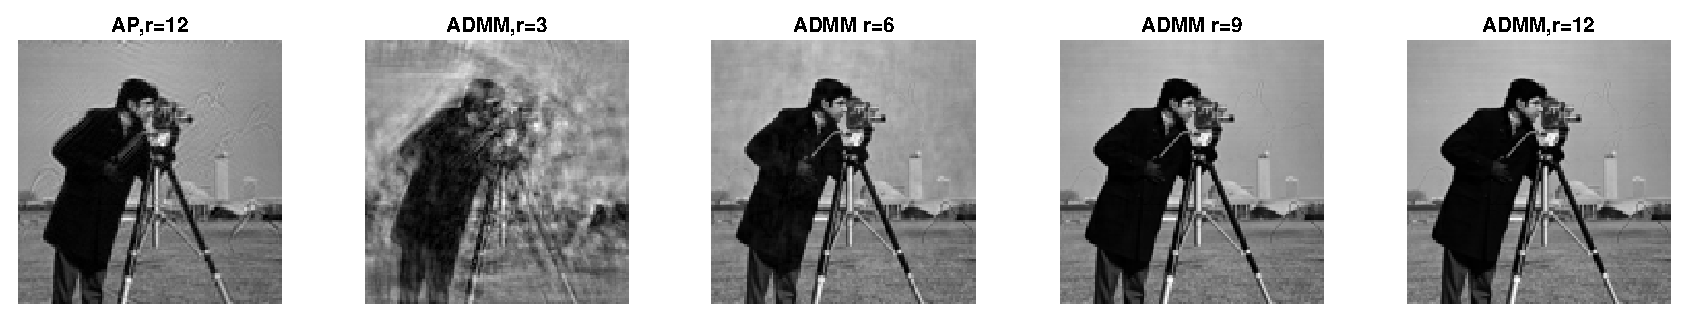
\includegraphics[width=0.9\linewidth]{figures/modes_u.eps}  
   \caption{Amplitude}
    \label{fig:modes_u}
 \end{subfigure}
 \begin{subfigure}{1\textwidth}
    \centering
    % include second image
    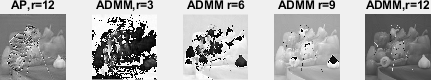
\includegraphics[width=.9\linewidth]{figures/modes_u_phaze.png}  
    %\caption{Put your sub-caption here}
    \caption{Phase}
    \label{fig:modes_u_phaze}
 \end{subfigure}
 
    \label{fig:modes_images}

 \end{figure}
 
 \begin{figure}[H]
 \begin{subfigure}{.5\textwidth}
    \centering
    % include first image
    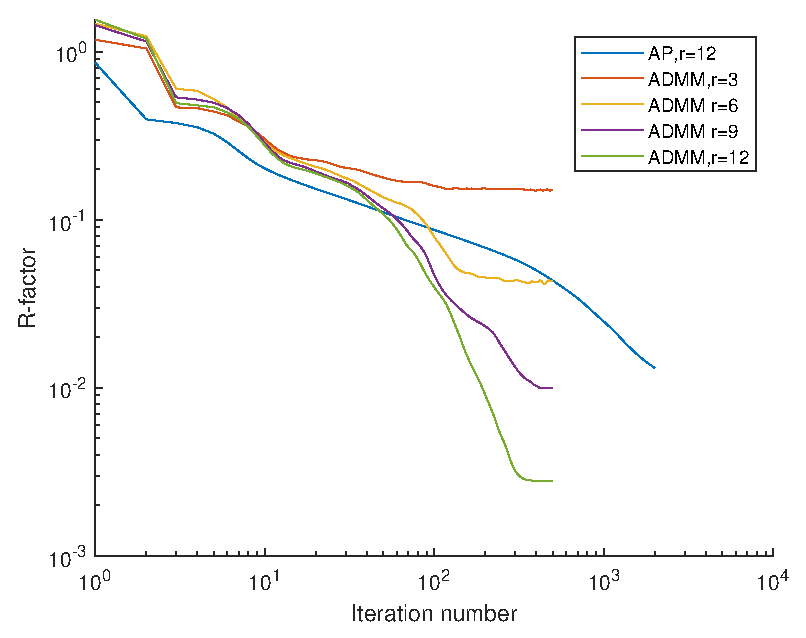
\includegraphics[width=0.9\linewidth]{figures/modes_R.eps}  
    %\caption{}
    \label{fig:modes_R}
 \end{subfigure}
 \begin{subfigure}{.5\textwidth}
    \centering
    % include second image
    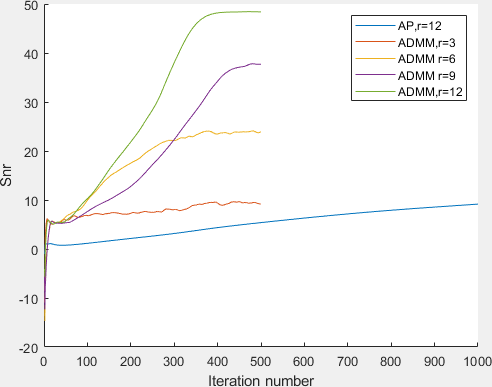
\includegraphics[width=.9\linewidth]{figures/modes_snr.png}  
    %\caption{Put your sub-caption here}
    \label{fig:modes_snr}
 \end{subfigure}
 \caption{R and snr. }
 \label{fig:noise}
 \end{figure}


We first compare $snr$ and $R$ for reconstructed images using a different number of modes. When the number of modes increases, the $R-factor$ decreases, and the $snr$ increases. That indicates that the quality of the reconstructed image increases.

The $R$ for 3,6,9,12 modes using ADMM algorithm are stable after 500 iterations at 0.15, 0.042, 0.0099, 0.0028, respectively, when $R$ for AP does not converge after 2000 iterations.


%fig2
\begin{figure}[H]
\centering
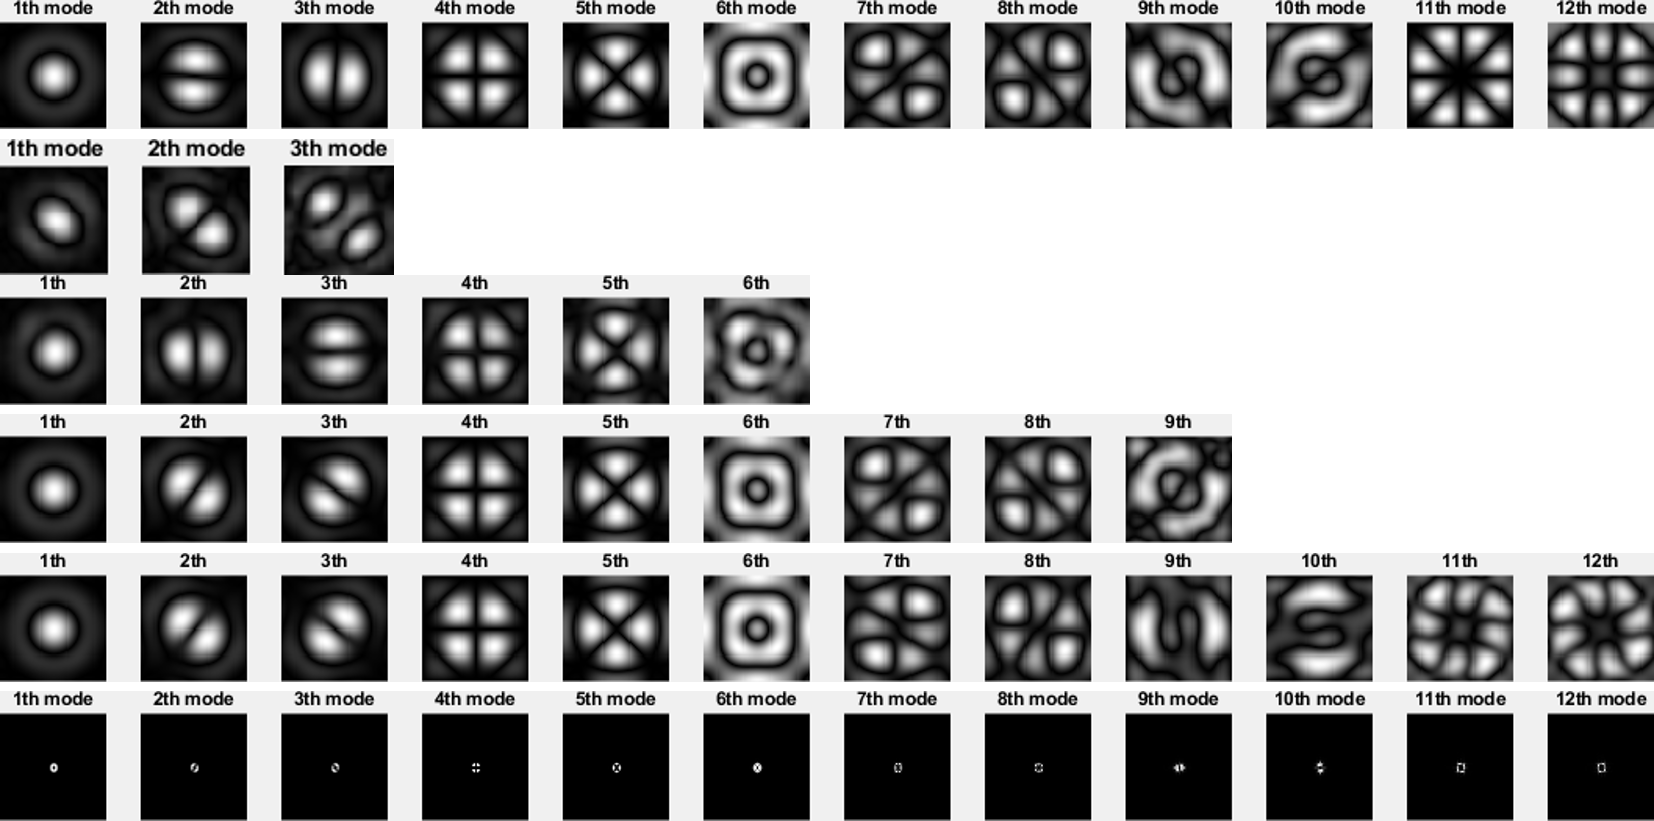
\includegraphics[width=1\linewidth]{figures/modes_combine}
\caption{Mode pattern. The first row represents the standard mode pattern. And the last two rows represent the mode pattern for 12 modes. Mode patterns are in the time domain except that the last row is in the frequency domain.}
\label{fig:modescombine}
\end{figure}

Standard mode pattern is obtained through performing SVD on standard density matrix generated from the model and extracting the first 12 modes. As shown in Figure \ref{fig:modescombine}, our algorithm can generally catch the main modes and get an optimal approximation.

%fig3 
Further, denote $err_M$ for r modes as $err_M^r$. Optimal $err_M^{r,*}$ can be calculated from the theory of low-rank approximation, and we compare our $err_M^r$ with it. Denote the singular values of standard density matrix $\rho_{true}$ as $s_i,i=1...d=rank(\rho_{true})$
 $$
 err_M^{r,*} = \min_{\rho, rank(\rho)=r} \dfrac{||\rho_{true} - \rho||_F}{||\rho_{true}||_F} = \sqrt{\dfrac{\sum_{i=r+1}^{d}s_i^2}{\sum_i s_i^2}}
 =
 \sqrt{1 - s_{cum}(r)}
 $$,
 $$
 where\ 
 s_{cum}(r) = \dfrac{\sum_{i=1}^{r}s_i^2}{\sum_i s_i^2} 
 $$
 
  %fig 4 approx fig 
 \begin{figure}
 \begin{subfigure}{.5\textwidth}
   \centering
   % include first image
   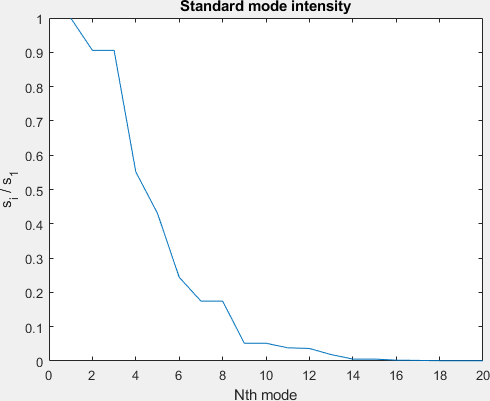
\includegraphics[width=0.9\linewidth]{figures/singular.png}  
   %\caption{}
   \label{fig:singular}
 \end{subfigure}
 \begin{subfigure}{.5\textwidth}
   \centering
   % include second image
   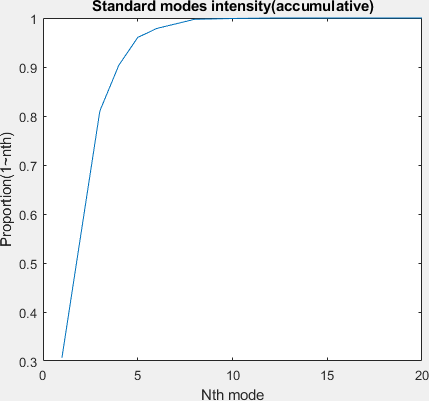
\includegraphics[width=.8\linewidth]{figures/singular_accumative.png}  
   %\caption{Put your sub-caption here}
   \label{fig:singular_acc}
 \end{subfigure}
 \caption{The distribution of singular values of the standard density matrix. The vertical axis in the left subfigure represents the ratio of $i^{th}$ largest singular to the first one $s_i/s_1$, and that in the right one represents $S_{cum}(i)$. The singular value decreases exponentially and the matrix is approximately low-rank. }
 \label{fig:standard singular}
 \end{figure}
 
 As shown in Figure \ref{fig:approx error}, the $err_M^*$ reaches around $0.01$, and $err_M$ is close to $err_M^*$ with 12 modes, which indicates that our algorithm does well in low-rank approximation to standard density matrix.

\begin{figure}[H]
\centering
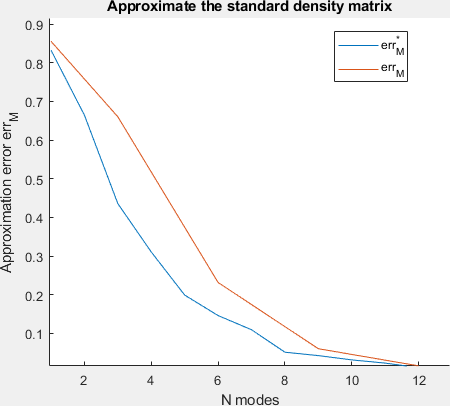
\includegraphics[width=0.8\linewidth]{figures/approximation.png}
\caption{}

   \label{fig:approx error}

 \end{figure}

\subsection{Add orthogonalization constraint}
The experiment setting is the same as above except that we change $ratio=\beta_2\beta$ to introduce orthogonalization constraint in ADMM. The larger the $\beta_2$, the stricter the orthogonalization constraint. As a reference, we also tried performing orthogonalization as in Algorithm \ref{alg:ort} every 20 iterations. 
%3
\begin{figure}
 \begin{subfigure}{.33\textwidth}
   \centering
   % include first image
   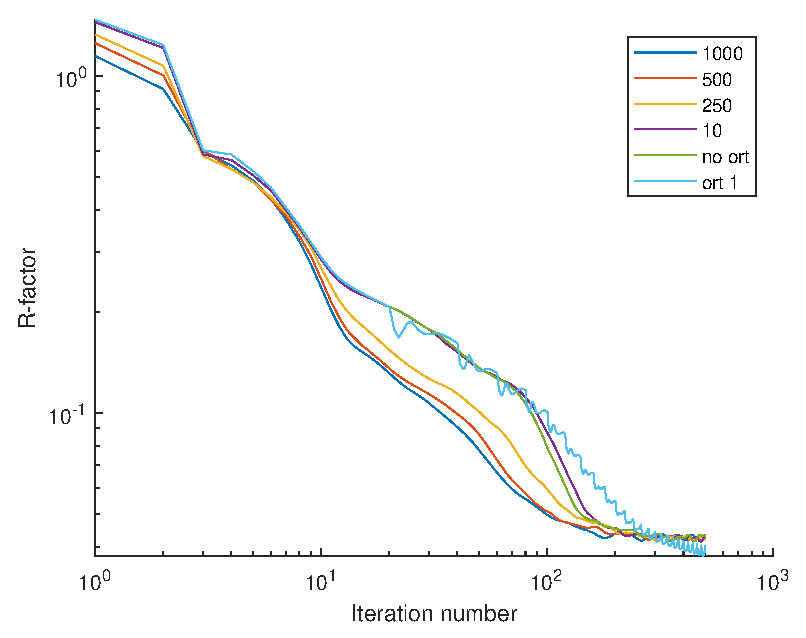
\includegraphics[width=1\linewidth]{figures/ort_R.eps}  
   %\caption{}
   \label{fig:ort_R}
 \end{subfigure}
 \begin{subfigure}{.3\textwidth}
   \centering
   % include second image
   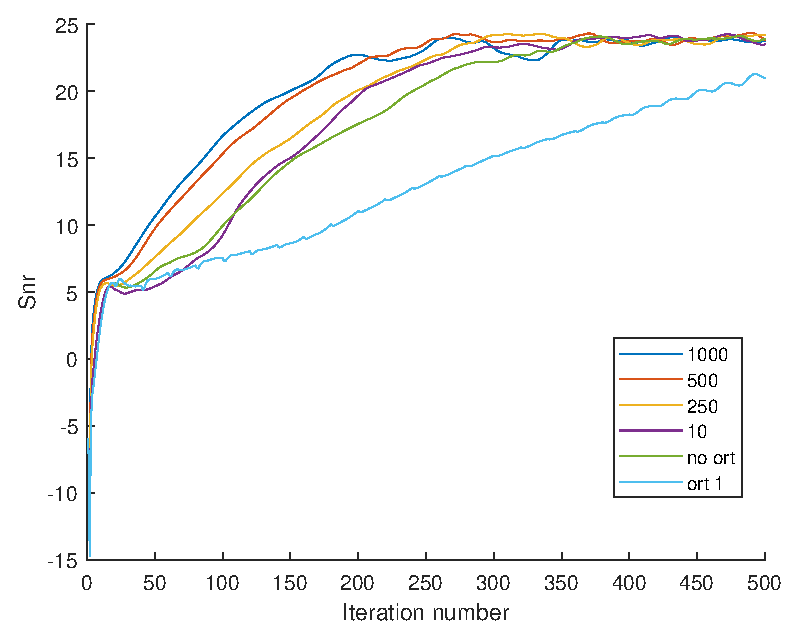
\includegraphics[width=1\linewidth]{figures/ort_snr.eps}  
   %\caption{Put your sub-caption here}
   \label{fig:ort_snr}
 \end{subfigure}
 \begin{subfigure}{.3\textwidth}
    \centering
    % include second image
    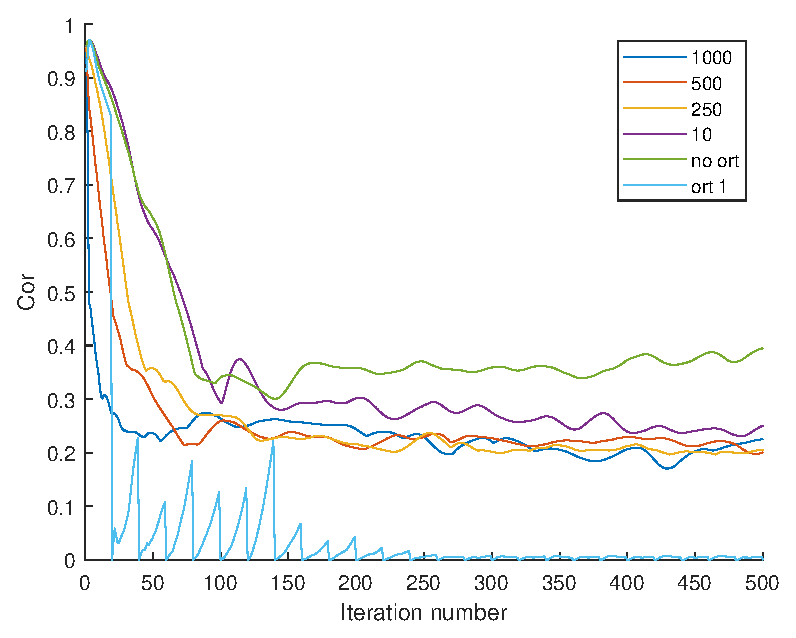
\includegraphics[width=1\linewidth]{figures/ort_cor.eps}  
    %\caption{Put your sub-caption here}
    \label{fig:ort_cor}
  \end{subfigure}
 \caption{The vertical axis and horizontal axis are set in log-scale in the first subfigure for R-factor. The blue line represents $\beta_2/\beta=1000$ and works the best in this case. The green line represents the result without orthogonalization. 'ort 1' means performing orthogonalization every 20 iterations. }
 \label{fig:ort}
 \end{figure}

 The reconstructed images are similar after 500 iterations, while $snr$ and $R factor$ using the ADMM algorithm with orthogonalization constraint improve faster. And the degree of correlation  $coherence$ between modes also decreases faster with larger $\beta_2$. 



\noindent\textbf{Remark.}

1. We suppose that orthogonalization constraints can improve robustness on different initial values. 

2. When the number of modes is large enough(like 12 here), the effect of the orthogonalization constraint seems not noticeable.

\subsection{Noisy case}
 $Dist=8$, $gridFlag=3$, $blurFlag=2$ and $\kappa$ is a guassian kernel with $\sigma = (15,15)$, $\beta=0.05$.
 
 Poisson noise is added on diffraction images $Y$ through MATLAB command:
 $$
  Y_{noise}=poissrnd(Y*(\eta))/\eta;
 $$
 where
 $\eta=0.0675$ is used here.
 
 Four different settings are compared: 9 modes with noise, 9 modes with noise, and 6 are kept after compression, 6 modes with noise, and 6 modes without noise(standard). Specifically, we conducted compression as in \ref{alg:compression} every 20 iterations, and kept 6 modes each time.
 
 %fig6 differet setting images, R, (snr without st)
 
 \begin{figure}[H]
 \centering
 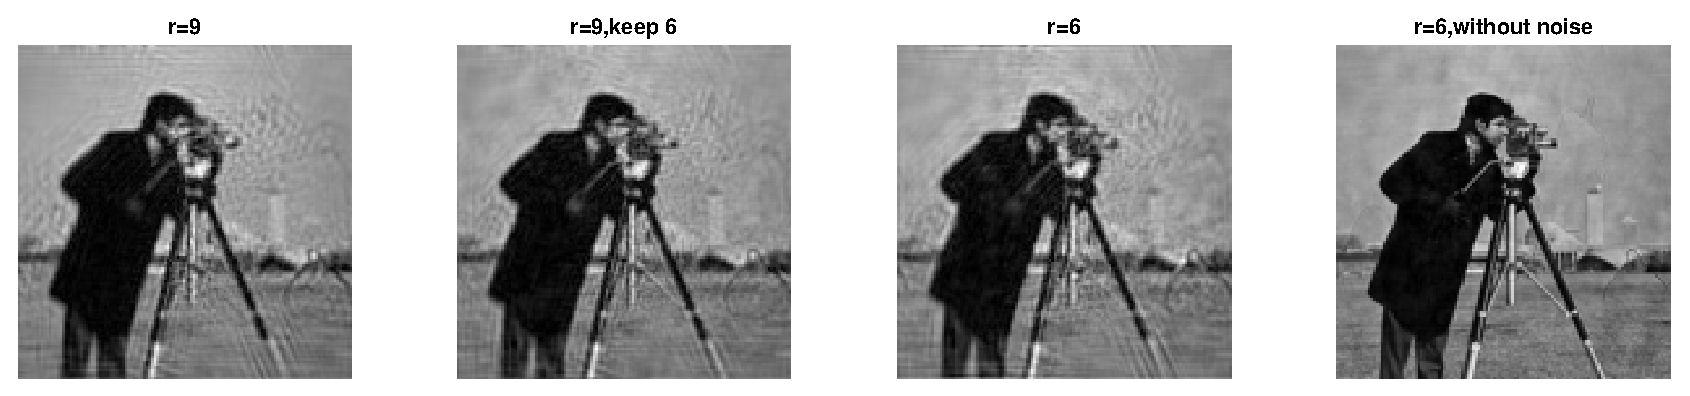
\includegraphics[width=1\linewidth]{figures/noise_u.eps}
 \caption{Reconstructed images in the noisy case}
 
    \label{fig:noise_u}
 
  \end{figure}
  
  \begin{figure}
  \begin{subfigure}{.5\textwidth}
    \centering
    % include first image
    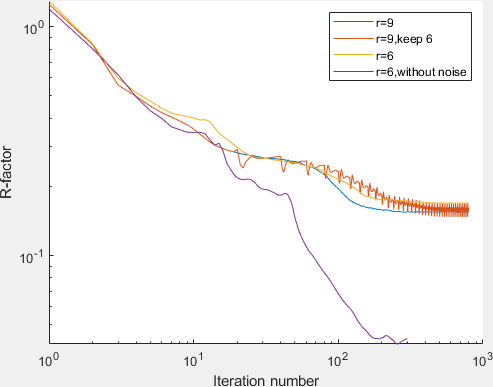
\includegraphics[width=0.9\linewidth]{figures/noise_R.png}  
    %\caption{}
    \label{fig:noise_R}
  \end{subfigure}
  \begin{subfigure}{.5\textwidth}
    \centering
    % include second image
    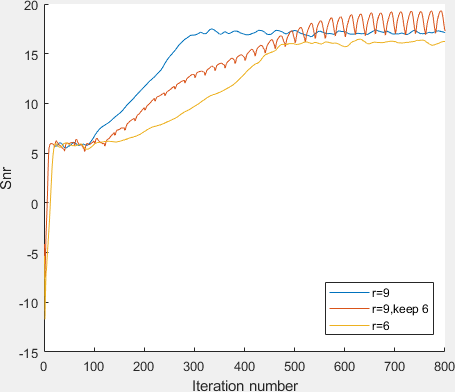
\includegraphics[width=.8\linewidth]{figures/noise_snr.png}  
    %\caption{Put your sub-caption here}
    \label{fig:noise_snr}
  \end{subfigure}
  \caption{R and snr. The red line represents the result with compression.}
  \label{fig:noise}
  \end{figure}
 
  The result periodically fluctuates with compression operation, while it can finally behave the best in the noisy case. Although the difference is not noticeable, we can consider adding compression in constraint instead of performing the direct truncated operation.
  
  \section{Appendix}
\subsection{Subproblems in ADMM}
\label{section:subproblems}
\subsubsection{$\omega$}
Essentially in this subproblem, each state $\omega_i=w(:,:,i)$ is independent. Then we can optimize each $w_i$ seperately.
 $$
 \omega_i^{k+1}=\arg \min _{\omega \in \mathcal{X}_{1}} \frac{1}{2} \sum_{j}\left\|\mathcal{F}^{-1} \hat{z}(:,:,j,i)^{k}-\omega(:,:,i) \circ \mathcal{S}_{j} u^{k}\right\|^{2}
 $$
 
 Essentially in this subsubproblem, each element in $w_i$ is independent.
 such that one just needs to solve the following 1D constraint quadratic problem:
$$
\omega_i^{k+1}(t)=\arg \min _{|x| \leq C_{\omega}} \rho_{t}^{k}(x).
$$
where
$\rho_{t}^{k}(x):=\frac{1}{2} \sum_{j}\left|\left(\mathcal{F}^{-1} \hat{z}(:,:,j,i)^{k}\right)(t)-x \times\left(\mathcal{S}_{j} u^{k}\right)(t)\right|^{2} \forall x \in \mathbb{C}$ 

The derivative of $\rho_{t}^{k}(x)$ is calculated 
\footnote{Notice that here $\rho$ is a real value function with complex variable, and we use wirtinger derivatives here. More properties and calculation rules are listed in this link: \url{https://blog.csdn.net/weixin_37872766/article/details/107673096}} as
$$
\begin{aligned}
&\nabla \rho_{t}^{k}(x) = \dfrac{ d\rho_{t}^{k}(x)}{dx^*} \\
&\begin{aligned}
=\sum_{j}\left(x \times\left|\left(\mathcal{S}_{j} u^{k}\right)(t)\right|^{2}-\left(\mathcal{S}_{j} u^{k}\right)^{*}(t)\left(\mathcal{F}^{-1} \hat{z}_{j,i}^{k}\right)(t)\right)
\end{aligned} \\
&\begin{aligned}
=x \times\left(\sum_{j}\left|\left(\mathcal{S}_{j} u^{k}\right)(t)\right|^{2}\right)-\sum_{j}\left(\left(\mathcal{S}_{j} u^{k}\right)^{*}(t)\left(\mathcal{F}^{-1} \hat{z}_{j,i}^{k}\right)(t)\right) \\
\end{aligned}
\end{aligned}
$$
The first order optimality condition is $\nabla \rho_{t}^{k}(x)=0 $. Then the close form solution of $w_i$ is given as
$$
\omega_i^{k+1}=\operatorname{Proj}\left(\frac{ \sum_{j}\left(\mathcal{S}_{j} u^{k}\right)^{*} \circ\left(\mathcal{F}^{-1} \hat{z}_{j,i}^{k}\right)}{ \sum_{j}\left|\mathcal{S}_{j} u^{k}\right|^{2}} ; C_{\omega}\right)
$$

 \subsubsection{z}
 $$
  \quad z^{k+1}=\arg \min _{z} \mathcal{G}(z)+\frac{\beta}{2}\left\|z-\mathcal{A}\left(\omega^{k+1}, u^{k+1}\right)+\Lambda^{k}\right\|^{2}\\
  $$
  $$
  =\arg \min _{z} \frac{1}{2}|| \sqrt{ \sum_{i=1}^{r} |z(:,:,:,i)|^2} - Y||^2+\frac{\beta}{2}\left\|z - z^+\right\|^{2}
 $$
 $$
 = \arg \min _{z} \sum_{x,y,j} [\frac{1}{2} ( \sqrt{ \sum_{i=1}^{r} |z(x,y,j,i)|^2} - Y(x,y,j) )^2 +
  \frac{\beta}{2}||z(x,y,j,:) - z^+(x,y,j,:)||^2 ]
 $$
 
 where $z^+ = \mathcal{A}\left(\omega^{k+1}, u^{k+1}\right) - \Lambda^{k}$
 
 For any fixed $x,y,j$ and free $i$, the problem can be seen as:
 
 $$
 z^*(x,y,j,:) = \arg \min_{z_{x,y,j} \in \mathbb{C}^{r}} \frac{1}{2} ( ||z_{x,y,j}|| - Y_{x,y,j} )^2
 + \frac{\beta}{2} ||z_{x,y,j} - z_{x,y,j}^+||^2
 $$
 
 Notice that for fixed $||z_{x,y,j}||$, the first term in expression is fixed. To optimize the second term, we should always choose $z_{x,y,j}$ with the same direction as $z_{x,y,j}^+$. So we have  $||z_{x,y,j} - z_{x,y,j}^+||^2 = (||z_{x,y,j}|| - ||z_{x,y,j}^+||)^2$
 $$
  \dfrac{z(x,y,j,i)}{||z_{x,y,j}||} = \dfrac{z^+(x,y,j,i)}{||z_{x,y,j}^+||}, z(x,y,j,i) = ||z_{x,y,j}||\dfrac{z^+(x,y,j,i)}{||z_{x,y,j}^+||}
 $$
 To determine $z_{x,y,j}$, we only need to determine $||z_{x,y,j}||$. Denote it as $a$.
 $$
 ||z_{x,y,j}||^* = \arg \min_{a \in \mathbb{R}} \frac{1}{2}(a - Y_{x,y,j})^2 + \dfrac{\beta}{2}
 (a - ||z_{x,y,j}^+||)^2
 $$
 The first optimality condition easily gives:
 $$
 a = \dfrac{Y_{x,y,j} + \beta ||z_{x,y,j}^+||}{1 + \beta}
 $$
 The  close form solution of Step 3 is given as:
 
 \begin{equation}
 z_i^{k+1} = \dfrac{z_i^k \dfrac{Y}{ M^k} + \beta z_i^+}{1+\beta}, 1 \leq i \leq r
 \label{zup}
 \end{equation}
 where $M^k =\sqrt{\sum_i |z^k(:,:,:,i)|^2} \in \mathbb{C}^{px \times py \times N}$
 
\subsubsection{D}

$$
\begin{aligned}
D^{k+1} =& \arg \min_{D} \| \Omega -  w^{k+1} + \Lambda_2^{k}\|^{2} \\
=& \arg \min_{D} \| D\alpha^k - \hat {w}^{k+1}\|^{2} 
\end{aligned}
$$
where $\hat {w}^{k+1} = reshape( \omega^{k+1} - \Lambda_2^{k},[px\times py,r])$,$D^*D=I$

This is a special case in Orthogonal Procrustes problem \footnote{\url{https://en.wikipedia.org/wiki/Orthogonal_Procrustes_problem}}
$$
\begin{aligned}
\| D\alpha^k - \hat {w}^{k+1}\|^{2} =& Tr[( D\alpha^k - \hat {w}^{k+1})^*( D\alpha^k - \hat {w}^{k+1})] \\
=& ||\alpha^k||_F^2 - Tr[(\alpha^k)^*D^*\hat{\omega}^{k+1}] - Tr[(\hat{\omega}^{k+1})^*D \alpha^k] + ||\hat{\omega}^{k+1}||_F^2
\end{aligned}
$$
$$
\begin{aligned}
D^{k+1} =& \arg \max_{D} Tr[(\alpha^k)^*D^*\hat{\omega}^{k+1}] + Tr[(\hat{\omega}^{k+1})^*D \alpha^k] \\
=& \arg \max_{D}  \Re{ (Tr[(\alpha^k)^*D^*\hat{\omega}^{k+1}] )}\\
\xlongequal{\alpha \in \mathbb{R}^{r\times r}}& \arg \max_{D}  \Re{ (Tr[D^* ( \hat{\omega}^{k+1}\alpha^k)]  )}
\end{aligned}
$$
Consider the SVD decomposition: $\hat{\omega}^{k+1}\alpha^k = USV^*$
$$
\begin{aligned}
D^{k+1} &= \arg \max_{D} \Re{ (Tr[D^*USV^*]  )}
= \arg \max_{D} \Re{ (Tr[(V^*D^*U)S]  )}\\
&\xlongequal{\hat{D} = V^*D^*U \text{ is orthonormal}}  \arg \max_{\hat{D}} \Re{ (Tr[\hat{D}S]  )}
\end{aligned}
$$
We can easily see $\hat{D} = I$ is optimal, and:
\begin{equation}
D^{k+1} = UV^*
\label{Dup}
\end{equation}



\begin{thebibliography}{99}
\bibitem{chang}{Chang, Huibin, et al. "Partially coherent ptychography by gradient decomposition of the probe." Acta Crystallographica Section A: Foundations and Advances 74.3 (2018): 157-169.}
\bibitem{theory}{Wolf E. New theory of partial coherence in the space–frequency domain. Part I: spectra and cross spectra of steady-state sources[J]. JOSA, 1982, 72(3): 343-351.}
\bibitem{mix}{Thibault P, Menzel A. Reconstructing state mixtures from diffraction measurements[J]. Nature, 2013, 494(7435): 68-71.}
\bibitem{direct}{Multiplexed coded illumination for Fourier Ptychography with an LED array microscope.}
\bibitem{algorithm}{Thibault P, Dierolf M, Bunk O, et al. Probe retrieval in ptychographic coherent diffractive imaging[J]. Ultramicroscopy, 2009, 109(4): 338-343.}
\bibitem{quan}{Introduction to Quantum Mechanics, David J. Griffiths, 12.3}
\bibitem{all}{Fannjiang A, Strohmer T. The numerics of phase retrieval[J]. Acta Numerica, 2020, 29: 125-228.}
\bibitem{admm}{Chang, Huibin, Pablo Enfedaque, and Stefano Marchesini. "Blind ptychographic phase retrieval via convergent alternating direction method of multipliers." SIAM Journal on Imaging Sciences 12.1 (2019): 153-185.}
\bibitem{psf}{Konijnenberg S. An introduction to the theory of ptychographic phase retrieval methods[J]. Advanced Optical Technologies, 2017, 6(6): 423-438.}
\end{thebibliography}






\end{document}